%-------------------------------------------------------------
%               FR CYBERDEF SECOPS COURSE
%                                        SECOPS
%                                            Intro
%
%                           Introduction Cyberdefense
%                            % Chap-Intro-gen.tex
%
%                              2020 eduf@ction
%-------------------------------------------------------------


\section{Avant propos}

Chaque jour la presse se fait l'écho d'attaques et de piratages informatiques, de divulgations d'informations sensibles ou  de fragilités découvertes dans les produits et services numériques.
Derrière ces incidents, nous découvrons des menaces certaines fois complexes, des actions criminelles, étatiques ou activistes. Construire des systèmes sûrs, les protéger et les défendre, dans une société où accélérer la digitalisation est devenu un challenge quotidien pour les équipes spécialisées qui luttent contre ces menaces. 
La cybersécurité est un domaine de mythes et de légendes. Ses activités plongent au plus profond de notre histoire avec des luttes ancestrales entre le méchant et le gentil, le gendarme et le voleur, le corsaire et le pirate, en n'oubliant pas les luttes secrètes entre les espions et le contre-espionnage. Une thématique qui résonne, donc comme un domaine de romans, qui se traduit toutefois par une réalité souvent moins réjouissante pour les équipes chargées de la cybersécurité dans les entreprises. Les métiers de la cybersécurité sont nombreux, pour certains très techniques, d'autres plus fonctionnels, juridiques, ou managériaux. 

La cybersécurité est, en effet,  une discipline transverse et interdisciplinaire à plusieurs titres. Elle nécessite  :
\begin{itemize}
  \item de maîtriser les nombreuses techniques et technologies des systèmes d'information ainsi que leurs zones de fragilités;
  \item de maîtriser de nombreuses solutions de sécurité permettant de couvrir, en n'oubliant qu'elles aussi peuvent être fragiles \footnote{cf. Certification et Qualification de produits de sécurité et Critères communs };
%\autoref{chap:ISOCC}

  \item de faire coopérer des métiers et des cultures différentes ;
  \item de gérer l'entreprise dans des cadres de conformité souvent complexes et coûteux;
  \item d'intégrer ces démarches en tenant compte des cultures et des pratiques des nombreux métiers de l'entreprise.
\end{itemize}

\mode<all>{\picframe{Tex/Pictures/img-4model}{Cybersécurité, un domaine hollistique}{0.9}{lbli4model}}

%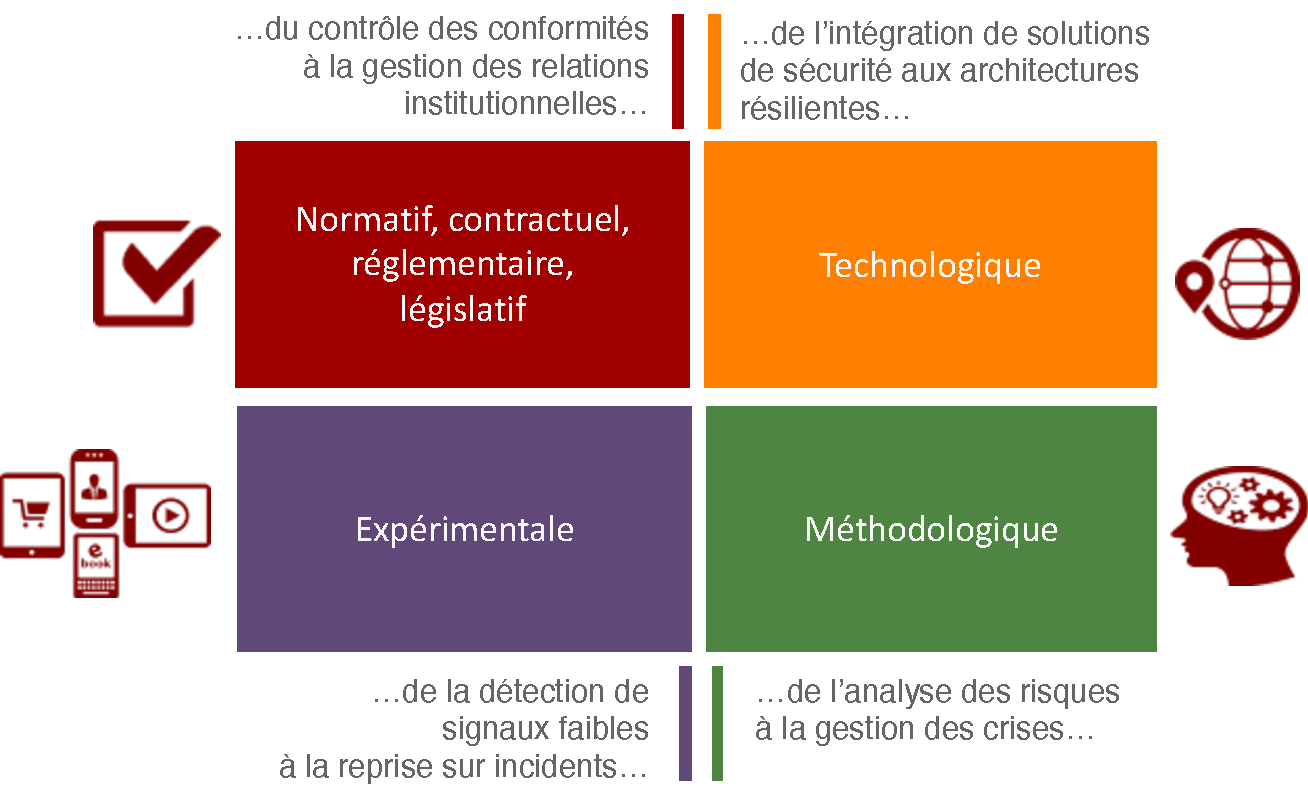
\includegraphics{Tex/Pictures/img-4model}

Les métiers de la cybersécurité concourent tous à une seule et même mission : \g{\textbf{assurer la continuité de la mission ou du service en préservant le patrimoine de l'entreprise contre toute menace dans l'environnement numérique}}.

Ce sont des métiers de passion, des métiers extrêmement techniques pour partie, fortement marqués par le fonctionnel pour d'autres. S'il est vrai qu'une grande partie des experts du domaine sont issus de formations en informatique ou en électronique, les domaines d'expertises s'élargissent et font naître de nouveaux chemins d'excellence. On trouvera en particulier, des métiers issus du domaine juridique comme celui du \uindex{Data Protection Officer}.    

%\section{les grands cyber-risques}

% les grands typologies de menaces liées au politique,, au vol, à la guerre économique" : Chantage, Images, Vole, Continuité d'activité ... manipulation, espionnage ...

% Les cyberrisques dependent de la cibles, et souvent la cible est liée à l'attaquant

%\section{les vecteurs cyber}

\section{Aborder la cybersécurité}

% ajouter le joke sur les corsaires et une hallebarde

La cybersécurité ou la sécurité du numérique\footnote{Historiquement d'autres termes sont utilisés comme  \ugls{aSSI} ou  Sécurité Informatique} peut être découverte par de nombreuses voies.

La plus courante est certainement pour les technophiles, l'aventure passionnante de découvrir ce domaine par la technique, et le hacking.  Longtemps abordé par le triptyque académique cryptologie,   sécurité  protocolaire des réseaux, et informatique fondamentale (compilation et théorie des langages, architecture système et bases de données), le domaine s'est vulgarisé avec une forme de gamification de l'apprentissage.

On y trouve en particulier :

\begin{itemize}
  \item Les challenges comme les \UKword{\ugls{aCTF}}, ou les \UKword{\ugls{aDTF}} qui permettent de mettre le pied dans les techniques et stratégies d'intrusion pour les pentesteurs et auditeurs techniques en herbe;
  \item Les bug-bounty qui permettent de se confronter à ses propres limites avec la recherche de failles dans les logiciels avec pour partie des rémunérations au niveau des difficultés;
\end{itemize}

Toutefois, un volet peu enseigné, qui ne mobilise pas spécialement les jeunes apprenants du domaine concerne la gouvernance de cette sécurité numérique de l'entreprise.

J'ai souhaité m'intégrer dans  une approche globale de la sécurité du numérique pas le biais de quelques processus, en particulier ceux de la sécurité opérationnelle. L'enjeu est de fournir une trame de connaissances pour déployer des actions de cybersécurité en entreprise.
Cette trame a pour intention de fournir des points d'accroche et des modèles de compréhension des différentes compétences, actions, et outils du large domaine de la cybersécurité.

Destiné à un public large, cet ouvrage tente d'offrir un niveau de lecture permettant à un expert technique de repositionner sa technicité dans un ensemble plus large, et  à un débutant de découvrir de nombreuses facettes du domaine avec quelques éclairages techniques.

La cybersécurité dans une entreprise est une co-activité d'hommes de l'art.  C'est aussi un domaine en perpétuelle évolution, soutenu et contraint par des lois, des règlements, des normes, des méthodologies,  des technologies spécialisées et en particulier des expertises.  Il nécessite pour être efficace d'être orchestré pour maintenir en condition de sécurité une organisation dont le périmètre peut être complexe face à des menaces elles aussi en perpétuelles évolutions.

Il y a de nombreuses manières d’aborder le pilotage de la cybersécurité au sein de l’entreprise, et nombreux ouvrages spécialisés en détaillent les concepts et les méthodologies. Nous avons toutefois délibérément choisi ici de confronter, si ce n'est de corréler, dans un seul support, trois domaines qui apparaissent souvent dans la littérature comme des domaines d'expertise différents : la gestion des risques, la gouvernance de la cybersécurité et la cybersécurité opérationnelle. 

Nous avons donc fait ce choix de structurer notre approche suivant le prisme de la cyberdéfense d'entreprise avec une analyse en trois axes majeurs qui résument les difficultés dont relève cette discipline holistique \ucite{sch13}. 


% begin PRZ===================
\begin{frame}{Les 3 axes de la cybersécurité}
	\begin{itemize}
 \item \tb{l'analyse des risques} informatiques sur les actifs les plus sensibles de l'entreprise avec les difficultés d'identifier ces actifs ainsi que leur sensibilité et les menaces qui pèsent sur ceux-ci ou sur l'environnement ;
\item la structuration d'une gouvernance efficace avec des \tb{politiques de sécurité} des systèmes d'information pour des architectures de sécurité de confiance, dans des systèmes d'information complexes, intégrant des services dans le cloud, des technologies obsolètes et des politiques de sécurité sédimentées ;
\item la construction et l’organisation d'une \textbf{sécurité opérationnelle} vue sous un angle d'anticipation et de veille, de détection, et enfin d'alerte et de réponse aux attaques, nécessitant une activité continue avec des ressources de plus en plus expertes et avec des outils plus \g{hyperspécialisés} et de plus en plus complexe à déployer.
\end{itemize}
\end{frame}
% end PRZ====================

%\rem{Politiques : le monde de la reflexion, Stratégies le monde l'action}
\subsection {Politiques versus stratégies}


\mode<all>{\picframe{Tex/Pictures/img-cycle}{Processus Cyber d'entreprise}{0.8}{lblcycle}}


Nous avons structuré la dynamique des processus d'entreprise dans c\edoc suivant un schéma simple\ uref{processus}{lblcycle}.
De  \head{l’analyse de risque}, nous pouvons déduire et/ou modifier des politiques de sécurité adaptées au contexte de l'entreprise. 
Sur la base de l’existant, il est alors possible d’adapter ou simplement de mieux utiliser ou configurer les architectures techniques et organisationnelles pour définir un niveau de protection attendu.
Il y a malheureusement toujours un écart entre les mesures de sécurité souhaitées et la réalité des mesures déployées. Que ce soit à cause de défauts de configuration, de délais de mise en place plus longs que prévu, le système n’est que très rarement au niveau décrit dans les éléments de spécification ou les documents d'assurance sécurité.
Mesurer ce niveau, analyser les écarts et remédier relève d’un des grands thèmes de la gouvernance sécurité. Il reste à lui seul un consommateur à plus de 30\% des charges d'activité de cette gouvernance.

Après avoir défini des \head{politiques de sécurité} et mesurer leur déploiement dans l’environnement de l’entreprise, il n’en demeure pas moins que l’ennemi est toujours à ses portes et de plus en plus souvent, il arrive à pénétrer le périmètre de sécurité.
Non pas que les barrières et filtre de l'entreprise ne soient plus efficaces mais simplement parce que l'attaquant change plus souvent de stratégie que l'entreprise de politique. La sécurité se doit donc d'être plus dynamique.
L’entreprise doit faire face à des attaquants qui ne raisonnent pas sous forme de politiques d’attaque, mais en stratégie d'action. L’entreprise doit raisonner aussi de la même manière pour se défendre. C'est à ce titre que l'on parle de stratégie de Cyberdéfense.
C'est avec des stratégies de \g{cyberdéfense} que nous aborderons les moyens organisationnels et techniques à mettre en place.

Vous trouverez  dans ce document une terminologie qui peut être certaines fois éloignée des expressions classiques de la sécurité informatique. \\
J'ai choisi d'utiliser et mixer sans trop de complexes des termes et concepts issus du monde militaire (renseignement, tenir une position, infiltration …) et de nombreux autres issus de l'univers médical (infection, épidémie, comportement).\\ Ces incursions dans les analogies d'autres champs professionnels, bien que présents pour illustrer certains concepts, n'en demeurent pas moins justifiés par leurs usages de plus en plus répandus dans le monde de la cybersécurité. Par ailleurs, les termes sécurité et cybersécurité pourront être utilisés indifféremment dans le corps de ce document.

\subsection {Transformation numérique}

% Les causes de la complexité

La cybersécurité est devenue en quelques années un axe fondamental dans la prise en compte de ces nouveaux risques sociétaux qu'apporte l'informatique au cœur de chaque activité sociale, économique ou politique.

%Quelque que soit le niveau d'impact  --- personnel, entreprise, Etatique, 
Les  transformations digitales d'une grande partie des acteurs économiques apportent de nouveaux risques. Les modifications des conditions d'utilisation des technologies dans les crises comme celle du COVID-19 engendrent aussi des risques globaux réduisant les frontières entre les espaces professionnels et les espaces privés.

Depuis bien des années, le législateur s'en est saisi avec de nombreuses réglementations et lois permettant de protéger en particulier, le citoyen et l'Etat.

On notera en particulier dans cette évolution du cadre réglementaire,  la protection des données personnelles, mais aussi la protection des systèmes sensibles stratégiques \footnote{\ugls{aOIV}  et \ugls{aOSE} } en lien avec la protection de la nation avec la dynamique de Cyberdéfense soutenue par les différentes lois de programmation militaire depuis 2008, et récemment la directive \ulink{https://www.ssi.gouv.fr/actualite/adoption-de-la-directive-network-and-information-security-nis-lanssi-pilote-de-la-transposition-en-france/}{NIS 2} . L'entreprise se trouve quant à elle prise en sandwich entre les exigences de l'état et les désirs de liberté que défend le citoyen. Il faut aussi noter que le salarié est souvent un citoyen et son rôle dans la cybersécurité de l'entreprise peut soulever des problématiques complexes\footnote{Lanceurs d'alertes, comportements déviants des utilisateurs légitimes}.
 
Se sentir en sécurité dans un monde de transformation digitale c'est bien entendu disposer des moyens de se protéger et protéger son patrimoine, que ce dernier soit ou non informationnel, mais aussi de le défendre en continu. Il est de moins en moins accepté de le protéger, en érigeant des murs épais, solides et supposés infranchissables. L'entreprise a besoin de faire circuler rapidement les savoirs, de partager largement des informations entre les salariés, les clients, les citoyens, les fournisseurs...


Il est donc nécessaire de correctement définir les biens vitaux ou essentiels pour y mettre les meilleurs moyens pour les défendre. Par ailleurs comme toute activité protégée et défendue qui peut subir des dommages, il est important de structurer l'activité numérique d'une entreprise ou d'une organisation pour pouvoir fonctionner en mode dégradé, et revenir à la normale en moins de temps possible.


Entre une maîtrise des risques cyber et une capacité de se défendre et réagir, il est nécessaire de disposer déjà d'un bon niveau de protection adaptée aux enjeux du numérique. Il existe de nombreuses définitions de cette cybersécurité.

Pour ma part je vous propose de poser pour la suite de mon propos, une définition simple, qui fait consensus et résume en une pseudo équation la manière dont nous traiterons ce domaine dans c\ecours. \\
\begin{nota}[Une définition de la cybersécurité]
\begin{align}
FORMULE RISQUE  MATH STYLE A MODIFIER
%Cybers\acute{e}curit\acute{e} \cong Cyberprotection\oplus Cyberd\acute{e}fense \oplus Cyberr\acute{e}silience
\end{align}
\end{nota}


% begin PRZ====================
\begin{frame}<presentation>{Une définition de la cybersécurité}
\begin{align}
Cybers\acute{e}curit\acute{e} \cong Cyberprotection\oplus Cyberd\acute{e}fense \oplus Cyberr\acute{e}silience
\end{align}
\end{frame}
% end PRZ====================

% begin PRZ====================
\begin{frame}

La cybersécurité est l'enchaînement opéré, organisé, documenté, piloté, optimisé de trois environnements d'actions :
\begin{itemize}
 \item \tb{Protéger} l'environnement par les mesures et solutions technologies adaptées au niveau de risque que l'entreprise est prête à prendre; 
 \item \tb{Défendre} les actifs les plus sensibles de l'entreprise en surveillant et combattant la menace (y compris l'image de l'entreprise);
 \item assurer \tb{la continuité et la reprise d'activité} de l'entreprise face à tout incident rendant indisponible tout ou partie d'une fonction essentielle de celle-ci.
\end{itemize}

\end{frame}
% end PRZ====================

La Cybersécurité, est donc, avant-tout, le déploiement de mécanismes de protection des biens et des processus numériques sensibles. C’est avec cette première dynamique que l’entreprise déploie en premier lieu des solutions de sécurité. 

Toutefois, malgré ce niveau de protection et souvent les lourds investissements réalisés dans des composants de sécurité périmètrique, l’entreprise peut se faire surprendre avec des attaques contournant ces mesures. Face à ces attaques, l’entreprise découvre que la solidité de l’entreprise n’est pas directement liée aux investissements sur les systèmes de protections. Il lui faut anticiper les menaces, les détecter non seulement sur son périmètre mais aussi dans l’écosystème de l’environnement des menaces potentielles. Ces menaces exploitent des vulnérabilités qu’il convient de détecter en amont.

Malheureusement, malgré ces mesures de protection et de défense qui permet de réagir vite et efficacement, il arrive que des attaques informatiques arrivent à leurs fins. La capacité de l’entreprise à revenir à une situation normale, avec un contexte assaini est un critère dont un chef d’entreprise appréciera la valeur \textbf{qu’après} un incident.

% ajouter l’equation du risque dans le texte du RISQUE

Il fut une époque pas si lointaine, où l'analyste consacrait beaucoup de temps à l'évaluation de la probabilité d'une attaque. Aujourd'hui bien que ce paramètre continue quand même à être pris en compte, l'analyste positionne cette probabilité ou \uindex{vraisemblance}
 à 100\% car pour l'entreprise la nouvelle hypothèse n'est pas de savoir "si un attaque va avoir lieu mais plutôt quand elle aura lieu" \uref{figure}{lblriskassess}.

% I M A G E -----------> 


\mode<all>{\picframe{Tex/Pictures/img-risk-assess}{le cyber-risque}{0.9}{lblriskassess}}

L'ensemble des experts du domaine est globalement en accord sur la posture que doivent prendre les entreprises et les organisations : \g{Le temps n'est plus de savoir si on sera attaqué ou pas, mais plutôt de savoir quand et comment on le sera}, qui concrètement se résume à la certitude que tout incident de sécurité peut se produire.

\mode<all>{\picframe{Tex/Pictures/img-risk-prison}{La menace, une vision de l'attaquant}{0.9}{lblriskjail}}

 
Dans les modèles d'analyse de risque et d'évaluation de la cybersécurité, l'analyste se positionne aujourd'hui du point de vue de l'attaquant. Ce regard lui permet de mieux comprendre la menace comme équation duale du risque, mais vu de l'énergie dépensée par l'attaquant et du risque qu'il prend \uref{figure}{lblriskjail}. La menace sera d'autant plus grand que la valeur des actifs visés est importante à ses yeux et que les vulnérabilités sont nombreuses. Elle sera d'autant plus faible que les moyens à déployer sont importants et les risques pris plus élevés.

On notera que la valeur des actifs visés dépend de l'attaquant. Ils ne seront pas les mêmes si l'attaquant est un état, une groupe d'activiste, un groupe criminelle.
Quand aux vulnérabilités, la majorité des attaques utilise les failles perpétuelles du facteur humain.




\section{Sécurité du système d'information}

Le système d'information est au coeur de ce \g{monde digital}, et il est le lieu d'activités humaines très denses, permettant à des utilisateurs de réaliser leurs activités, professionnelles ou privées, à l'aide de processus informatiques et de services. 

Ces activités doivent de plus en plus faire face à tout un système d'agression orchestré par des attaquants non seulement humains mais aussi \g{automatiques}. On observe aujourd'hui une multitude de situations critiques, incertaines dont l'occurrence quasi quotidienne provient de phénomènes variés, humains (isolés, en réseau, …), physiques et/ou technologiques. Parmi ces difficultés qui profitent aux pirates informatiques il y a de nombreuses failles ou fragilités que nous découvrirons, provenant des systèmes du SI sans lesquelles ils ne pourraient exploiter leurs attaques. Ces phénomènes sont une menace pour les conditions de sécurité du système d'information.


\subsection{Gouvernance et conformité}

\utodo

\subsection{SECOPS et lutte contre la malveillance}

\utodo

\subsection{Les fonctions SSI de gouvernance}

Au sein des grandes entreprises, il existe de nombreuses fonctions ou missions pour gouverner, piloter cette sécurité numérique.

%----begin FRAME-------
\mode<all>{\texframe
{SSI : Responsabilités}
{les métiers}
{
\begin{itemize}
 \item \head{Le gestionnaire de risque} ou \UKword{Risk Manager} qui porte l'animation de la gestion des risques dans les projets ou dans l'entreprise;
\item \head{Le responsable sureté / sécurité } généralement responsable de la sécurité physique ou sein de l'entreprise (vol, intrusion physique, contrôle d'accès). Il endosse le plus souvent la responsabilité des biens et des personnes;
\item \head{L'audit et le contrôle} : Au sein des grandes organisations, il peut exister un service \g{indépendant} dont la mission est d'auditer et de contrôler les activités des services;
\item \head{Les RSSI} : Responsables de la sécurité des Systèmes d'Information;
\item \head{Les DSSI} : Au sein des grandes entreprises, les RSSI globaux ne dépendent plus trop de DSI, et possèdent le rang de directeur;
\item \head{Le DPO} : la dernière responsabilité apparue dans l'environnement de la sécurité (En France successeur du CIL , Correspondant Informatique et Liberté) (\UKword{Data Protection Officer}).
\end{itemize}
}}%----end FRAME-------


Nous ne présentons rapidement ici que ceux qui seront utilisés directement dans ce document et qui sont fortement en liaison avec la sécurité des systèmes d'information.

\subsubsection{Les DSSI et RSSI}

Au sein de l'entreprise, il est important que quelqu'un porte la charge de suivre ces conditions de sécurité. C'est le rôle du RSSI (Responsable de la sécurité des systèmes d'information), ou DSSI (Directeur de la sécurité des systèmes d'information).
La mission de ce RSSI d'entreprise est de protéger son Système d'Information (SI), de le mettre dans une posture d'amélioration continue tant de son système de protection que de son système de défense. Le RSSI n'est pas seul pour assumer ces missions, à tous les niveaux de l'entreprise, s'organise des fonctions de sécurité tant au sein de la DSI (auquel est souvent rattaché le RSSI), qu'au sein d'autres activités de l'entreprise. 

\subsubsection{Le DPO}

A partir de mai 2018, une responsabilité plus juridique liée à la protection des données a été rendue plus visible avec la nécessité de disposer d'un \ugls{aDPO} en entreprise (Data Protection Officer) héritier en France  \textit{\ugls{aCIL}}.
Nous n'aborderons pas la fonction, les missions et la dynamique de responsabilité du \ugls{aDPO} ici. Il faut toutefois que cette fonction possède de nombreux recouvrements dans la chaine de gouvernance du risque \g{informatique} auprès des directions d'entreprise. Orienté vers la protection des données à caractère personnel, le tropisme de la fonction \ugls{aDPO} peut conduire certaines structures à oublier des pans importants des risques numériques comme :

\begin{itemize}
	\item la protection du patrimoine informationnel. (Espionage industriel).
	\item la protection des systèmes d'information contre les risques de ruptures de services (Continuité d'activité)
\end{itemize}

\subsubsection{L'officier de sécurité de défense}
Pour les entreprises traitant des informations classifiées de défense ou liées aux contraintes de la classification de l'état, il est indispensable de se doter d'une fonction \ugls{aOS} de défense. Son rôle est de s'assurer de la conformité à l'Instruction Générale Interministérielle IGI 1300 pour le \g{Confidentiel Défense} et l'instruction Interministérielle II901 pour le \g{Diffusion Restreinte}.

Nous resterons donc dans le cadre fonctionnel de la Cybersécurité dans son volet protection des Systèmes d'information et gestion des risques numériques.
Quand nous aborderons des sujets en forte adhérence avec les dynamiques de la \ugls{aGDPR} nous donnerons les liens et les indications adaptés pour les \ugls{aDPO}.
Par exemple, nous aborderons l'usage des données nominatives collectées et traitées dans les \ugls{aSIEM}, ou celles recueillies sur le DarkWeb etc ...

Consulter le site de la \ulink{www.cnil.fr}{CNIL} pour parfaire ses connaissances en matière de réglementation européenne sur la protection des données personnelles. 


\subsubsection{Responsabilités SSI}

Le maintien des conditions de sécurité du système d'information des grandes entreprises nécessite un \ugls{aRSSI} Central ou une fonction semblable rattachée à un niveau plus global de l'entreprise.
On découvre ainsi des  \ugls{aRSSI} rattachés à la direction des risques, la direction générale, au contrôle interne …\\
 Il n'y pas de rattachement bien défini. La couverture de responsabilité dépend grandement de la taille et de l'activité de l'entreprise, mais aussi de la maturité de celle-ci en matière de gestion de risque et de gouvernance. Il peut y avoir des RSSI par entité, par projet à l’intérieur d'une entreprise. Leur mandat est fixé en fonction des enjeux sécurité de ces entités ou ces projets. 

Le fin mot de l'histoire est le \g{R} de  \ugls{aRSSI}. Son domaine de responsabilité dépendra de son mandat pour assumer ce rôle de garant d'un environnement \g{possédant } des bonnes conditions de sécurité.
La gouvernance de la sécurité, est au coeur du métier du  \ugls{aRSSI}. Cette discipline que ce dernier pilote dans l’entreprise se nomme \ugls{aGRC}.

La notion de système d'information a profondément évoluée ces dernières années. Le périmètre des risques digitaux inclut maintenant des systèmes et services externes à l'entreprise. Beaucoup d'entre eux sous la forme de réseaux sociaux, de services \uindex{cloud}
 ouvrant par ailleurs le domaine de supervision à la téléphonie avec les smartphones et leurs applications professionnelles ou non.

Bien entendu en fonction de la taille de l'entreprise et de ses enjeux, on peut disposer au sein de l'entreprise de nombreuses personnes ayant une fonction de \ugls{aRSSI}. 

Le métier est riche et dispose d'un spectre de responsabilité et d'activité très large en terme de poste on y trouve par exemple :

% FRAME beamer PRZ ------------------------------------
\mode<all>{\texframe{Fonctions RSSI}{différents métiers} 
{
\begin{itemize}
\item \textbf{RSSI d'entreprise} : Responsable de la sécurité de sa structure.
\item  \textbf{RSSI d'un département, d'une organisation intermédiaire} : A l'image d'un RSSI d'entreprise, il assure toute les tâches de gouvernance, il applique et fait appliquer les directives et politique de sécurité aux équipes du département / division / structure intermédiaire, il déploie les actions décidées dans la chaîne fonctionnelle sécurité
\item   \textbf{RSSI d'un contrat, d'un projet contractualisé (Security Manager)} : Responsable de la sécurité du  déroulement d'un contrat. Souvent lié à un plan d'assurance sécurité, le RSSI contrat se doit d'assurer pour le client ou pour le fournisseur le suivi des exigences de sécurité du contrat.
\end{itemize}
}} % end FRAME.........................................................


\mode<all>{\texframe{Fonctions RSSI}{suite}
%. . . . . . . . . . . . . . . . . . . . . . . . . . . . . . . . . . . . . . . . . . . .
{\begin{itemize}
	\item \textbf{RSSI Projet} : La responsabilité sécurité couvre le projet, on parle souvent de \g{\uindex{security by design}
}. La responsabilité dans ce type de poste recouvre l'intégration de la sécurité dans le système, le suivi des indicateurs définis (contractuels, ou réglementaires), la remontée des indicateurs de suivi de sécurité à la MOA (Maitrise d'ouvrage), la prise de décision autour des choix de sécurité ....
	\item \textbf{RSSI Produit / Service} : Au delà de ce qui est fait pour un projet, le RSSI produit a en charge de gérer la sécurité opérationnel c'est à dire Maintenir la sécurité de son produit ou de son service.
 \item \textbf{RSOP} : Le responsable sécurité opérationnelle, est souvent un RSSI dépendant d'une DSI, il est généralement et dans beaucoup de d'entreprise de taille moyenne le RSSI technique. Il assure opérationnellement la mise en place technique des politiques de sécurité et maintien en condition de sécurité l'ensemble de l'environnement informatique. Il est aujourd'hui au coeur de la sécurité opérationnelle face aux attaques et aux crises cyber.
\end{itemize}
}} % end FRAME.........................................................


\subsection{Maintien en condition de sécurité}

Les conditions de sécurité représentent les propriétés fondamentales du SI, appelées : \ugls{aDICT} , qui favoriseront le fonctionnement optimisé du SI et éviteront l'avènement d'incidents de sécurité irréversibles ou même gênants pour son fonctionnement. D'un certain point de vue, les conditions de sécurité représentent le paramétrage du SI pour lequel le système fonctionne bien dans des conditions de sécurité \g{connues et approuvées}.

Ces fameux critères \textbf{\ugls{aDICT}} ou propriétés de sécurité des systèmes d'information visent les objectifs suivants :
%-----------------------------------------
\begin{nota}[DISPONIBILITE]
le système doit fonctionner sans faille (arrêt, ou dégradation) durant les plages d'utilisation prévues et garantir l'accès aux services et ressources définies et installées avec le temps de réponse attendu.
\end{nota}
%-----------------------------------------
\begin{nota}[INTEGRITE]
Les données doivent être celles que l'on attend, et ne doivent pas être altérées de façon fortuite, illicite ou malveillante. En clair, les éléments considérés doivent être exacts et complets.
\end{nota}
%-----------------------------------------
\begin{nota}[CONFIDENTIALITE] Seules les personnes autorisées peuvent avoir accès aux informations qui leur sont destinées. Tout accès indésirable doit être empêché.
\end{nota}
%-----------------------------------------
\begin{nota}[TRACABILITE] (ou preuve ) : garantie que les accès et tentatives d'accès aux éléments considérés sont tracés et que ces traces sont conservées et exploitables.
\end{nota}
%-----------------------------------------
D'autres aspects peuvent aussi être considérés comme des objectifs de la sécurité tels que :
%-----------------------------------------
\begin{nota}[AUTHENTICITE]
l'identification des utilisateurs est fondamentale pour gérer les accès aux espaces de travail pertinents et maintenir la confiance dans les relations d'échange. On voit aussi dans la littérature la terminologie \g{critères \ugls{aACID} (Authentification, Confidentialité, Intégrité, Disponibilité)}.
\end{nota}
%-----------------------------------------
\begin{nota}[NON-REPUDIATION]
La non-répudiation et l'imputation : aucun utilisateur ne doit pouvoir contester les opérations qu'il a réalisées dans le cadre de ses actions autorisées et aucun tiers ne doit pouvoir s'attribuer les actions d'un autre utilisateur.
\end{nota}

Dans un contexte d'activité économique dense et en perpétuel renouvellement, les conditions de sécurité sont aussi en perpétuelle évolution, c’est pourquoi nous parlons d'un cycle de vie vertueux au cours duquel les nouveaux paramètres tirent profit des expériences passées.  Ainsi, l’amélioration continue également appelée \g{ lean management} dans d’autres domaines (industrie, …) travaille elle sur le cycle de vie des conditions de sécurité souvent appelé \ugls{aPDCA}.\\
Ce cycle de vie doit néanmoins être maitrisé par le RSSI en place avec ses équipes, il faut co-produire ces conditions de sécurité, cette maîtrise est complexe, fortement dépendante du contexte de l'entreprise, c’est pourquoi elle doit être accompagnée d'une méthodologie rigoureuse et partagée qui constitue le savoir-faire de base du RSSI et de son équipe. Par ailleurs, parmi ces conditions, certaines sont universelles et d’autres propres à chaque entreprise. \\ Comme le montre le cycle de vie. \uref{diagramme}{lblcycledevie}, il est possible aussi d’utiliser un cycle de vie sécurité de type projet, qui se rapproche par ailleurs de la manière dont nous avons structuré c\edoc. 

\mode<all>{\picframe{Tex/Pictures/img-cyclevie}{Cycle de vie sécurité dans les projets}{0.9}{lblcycledevie}}


Dans cette optique, ce cadre méthodologie a été défini par le sous-comité 27 de l'ISO, par l'ensemble de normes ISO 27x. Il s’agit également d'un ensemble de bonnes pratiques, qu'un RSSI peut suivre au travers de trois volets fondamentaux qui constituent les référentiels utilisés pour ce cours sur la cybersécurité. La norme 27001 est en particulier un cadre pour organiser la dynamique de la mise en condition de sécurité de l’entreprise et son maintien dans le temps. Cet environnement que le \g{RSSI} doit bâtir est le système de management de la sécurité (\g{SMSI}).\\
Notre dynamique méthodologique est soutenue dans  c\edoc, par trois cadres normatifs : 
 
% FRAME beamer PRZ ------------------------------------
\mode<all>{\texframe{Cadres normatifs}{3 modèles du cadre}
%. . . . . . . . . . . . . . . . . . . . . . . . . . . . . . . . . . . . . . . . . . . .
{
\begin{itemize}
\item Identifier ses cyber-risques sur la base de méthodologies que l’on retrouve dans l’environnement ISO/CEI 27001/27005 mais aussi sur la méthodologie \ugls{aEBIOS} de l’ANSSI (Méthode \ugls{aEBIOS} RM en particulier); 
\item Elaborer une politique de cybersécurité sur la base des cadres ISO/CEI  27001 et 27002, en n’oubliant pas les architectures de sécurité et la sécurité des architectures associées ; 
\item Détecter en amont des attaques et savoir réagir à ses cyber-incidents en se basant sur ISO 27035 et sur la continuité d’activité avec l’ISO 22301 et 27031.
\end{itemize}
}} % end FRAME.........................................................


\begin{nota}[Pourquoi des normes dans c\edoc?]
L’objectif de c\edoc, n’est pas de présenter en détail un cadre normatif, mais bien de les utiliser pour ce qu’elles sont : des langages communs permettant d’appréhender une terminologie, des méthodologies, des outils. L’ISO 27001 comporte un grand nombre de normes (plus de 50…) qu’il convient de connaître comme outils terminologiques et de référence. Leur maîtrise nécessite une spécialisation le plus souvent demandée pour des métiers de conseil ou d’implémentation pour une certification.
\end{nota}

Ces documents définissent un cadre méthodologique et normatif pour définir, créer, élaborer maintenir, améliorer les conditions ou les critères de sécurité pour le fonctionnement du système protégé et surveillé. 
Ils permettent aux acteurs de l'entreprise évoluant autour du métier RSSI un cadre méthodologique ainsi qu’un \g{how to} du maintien en conditions de sécurité. C’est en particulier au travers de ces trois axes que la mission de RSSI repose. 
Le nombre d’entreprises prêtes à accueillir des spécialistes de ce savoir-faire est en forte augmentation car les PME/PMI ont pris conscience que la sécurisation de l’entreprise est devenu primordiale pour \g{survivre} dans l’écosystème digital de nos sociétés modernes. Les contraintes légales issues de la Loi de Programmation Militaire (\ugls{gLPM}), de la Règlementation pour la Protection des Données Personnelles (RGPD), de la directive NIS nécessitent de disposer d’une vision globale et transverse tant technique, qu'organisationnelle ou humaine de la cybersécurité.

Nous tenterons donc dans le suite du cours, de vous donner des contextes d'usages de ces cadres normatifs indispensables pour aborder la cyberdéfense d’entreprise. 

\section{Enjeux légaux}

Beaucoup d'environnements normatifs sont issus de la pression des différents cadres législatifs sur le marché. Que ce soit avec la pression du grand public ou avec les enjeux stratégiques et économiques des pays, ces lois organisent profondément les modes de gouvernance de la sécurité en entreprise.

\subsection{Quelques cadres législatifs d'influence}
Parmi les grandes lois qui ont influencées  le monde de la sécurité des entreprises ces dix dernières années :

\begin{itemize}
 \item En France, le cyberdéfense est largement orientée par les différentes \g{Lois de programmation militaire} avec des directives nationale de sécurité par grands domaines d'infrastructures vitales.
 \item En Europe deux grandes directives ont donné plus de responsabilités aux entreprises dans l'engagement sécurité avec GDPR et NIS qui sont déclinés en droits français via la CNIL, et l'ANSSI. On notera par ailleurs la montée en puissance dans la confiance numérique avec le cadre de certification européen.
 \item Aux Etats Unis, le \UKword{Cloud security Act}, a bouleversé la vision des risques numériques des états avec les potentielles nuisances liées à l'extraterritorialité de lois américaines
 \item En Russie et en Chine, plusieurs lois autour de l'usage d'internet interpellent les entreprises et en particulier celles du numérique sur la protection des données de leurs clients ou utilisateurs de leurs services.
\end{itemize}


\subsection{Le cadre de certification européen}

Le règlement établit un \ulink{https://www.ssi.gouv.fr/entreprise/reglementation/cybersecurity-act-2/le-cadre-de-certification-europeen}{cadre européen de certification}
 de cybersécurité pour harmoniser à l’échelle européenne les méthodes d’évaluation et les différents niveaux d’assurance de la certification, au sein duquel l’ENISA trouve toute sa place. Les certificats délivrés bénéficieront d’une reconnaissance mutuelle au sein de l’Union européenne (UE). 

\subsection{Cyberdefense et loi de programmation militaire}
Pour ceux intéressés par les contraintes et cadres généraux de la cyberdéfense au sein des lois de programmation successives (2008, 2013, 2019 ...) il est conseiller d'aller voir sur le site de l'ANSSI. Les différentes LPM ont fait évoluer le cadre réglementaire pour assurer à la France une capacité de défendre la continuité de l'état et des infrastructures vitales du pays \ulink{https://www.ssi.gouv.fr/entreprise/protection-des-oiv/protection-des-oiv-en-france/}{(Cf. Opérateurs d'infrastructures vitales)}.
